\documentclass[11pt]{article}
\usepackage[margin=1in]{geometry}
\usepackage[T1]{fontenc}
\usepackage{amsmath,amssymb,amsthm,mathtools}
\usepackage{graphicx}
\usepackage{xcolor}
\usepackage[hidelinks]{hyperref}
\usepackage{microtype}

\newtheorem{theorem}{Theorem}
\newtheorem{lemma}[theorem]{Lemma}
\newtheorem{corollary}[theorem]{Corollary}
\newtheorem{remark}[theorem]{Remark}
\newcommand{\R}{\mathbb R}
\newcommand{\N}{\mathbb N}
\newcommand{\eps}{\varepsilon}

\title{A rotund, G\^ateaux-smooth, nowhere-LUR renorming\\
for spaces with complemented $\ell_1$}
\author{Candidate partial-result packet for arXiv:2402.13869}
\date{11 August 2026}

\begin{document}
\maketitle

\begin{center}
\fbox{\begin{minipage}{0.91\textwidth}
\textbf{Status.} Candidate substantial partial result, likely valid, pending
expert review.  The theorem below answers Problem~3.7 of
De~Bernardi--Preti--Somaglia for every separable real Banach space containing
a complemented copy of $\ell_1$.  It does not settle the problem for arbitrary
separable Banach spaces.
\end{minipage}}
\end{center}

\section{Source problem and evidence}

The source is C.~A. De~Bernardi, A.~Preti, and J.~Somaglia,
\emph{A note on smooth rotund norms which are not midpoint locally uniformly
rotund}, arXiv:2402.13869 \cite{DPS}.  Problem~3.7 on PDF page~9 asks:
\begin{quote}
Can every infinite-dimensional separable Banach space be renormed to be
rotund [and G\^ateaux smooth] but with no LUR point in the unit sphere?
\end{quote}
The original page is reproduced below.  The full-width crop includes the
problem label, complete statement, and immediate context.

\begin{center}

\includegraphics[width=\textwidth]{figures/open_problem_crop.png}
\end{center}

The source records positive results for spaces containing $c_0$ and for
polyhedral spaces, and proves that every separable infinite-dimensional space
has a rotund G\^ateaux-smooth norm which is not MLUR at at least one point
\cite{DPS}.  The result here supplies a different broad positive class and,
within that class, eliminates \emph{all} LUR points while retaining both
rotundity and G\^ateaux smoothness.

\section{Definitions}

A norm $p$ is \emph{rotund} (strictly convex) if equality
$p(x+y)=p(x)+p(y)$ for nonzero $x,y$ forces $x$ and $y$ to be positive scalar
multiples.  A point $x\in S_{(X,p)}$ is \emph{LUR} if, whenever
$x_k\in S_{(X,p)}$ and $p(x+x_k)\to2$, one has $p(x-x_k)\to0$.

A norm $p$ is \emph{octahedral} if for every finite-dimensional
$F\subset X$ and every $\eps>0$ there is $u\in S_{(X,p)}$ such that
\[
 p(y+\alpha u)\ge (1-\eps)\bigl(p(y)+|\alpha|\bigr)
 \qquad(y\in F,\ \alpha\in\R).
\]
An octahedral norm has no LUR points; a short proof is included below.

\section{Proof Intuition}

Cobollo and H\'ajek constructed a G\^ateaux-smooth octahedral norm $N$ on
every space with a complemented $\ell_1$, provided the space admits some
G\^ateaux-smooth norm \cite{CH}.  Their construction does more than assert
octahedrality: relative to a decomposition
$X=X_0\oplus\ell_1$ and its canonical vectors $e_n$, it gives a uniform
asymptotic $\ell_1$ estimate for $P_{n-1}x+\alpha e_n$.

Adding an ordinary \emph{equivalent} strictly convex norm to $N$ would charge
every normalized $e_n$ by a fixed positive amount and could destroy that
estimate.  Instead, we build a continuous injective strictly convex smooth
norm $h$ which is deliberately non-equivalent and satisfies
$h(e_n)=2^{-n}\to0$.  Then
\[
                         M=N+h
\]
is still equivalent because $N$ is, is rotund because equality for $M$ forces
equality for the strictly convex summand $h$, and is G\^ateaux smooth because
both summands are.  The exact Cobollo--H\'ajek tail estimate shows, with no
compactness guesswork, that the normalized $e_n$ remain octahedral witnesses
for $M$.  Octahedrality then supplies, at every unit vector $x$, unit vectors
$u_k$ for which both $M(x+u_k)$ and $M(x-u_k)$ tend to $2$, ruling out LUR at
$x$.

The unresolved part of the source problem remains substantial: spaces not
containing $\ell_1$ admit no octahedral renorming at all, so a full answer must
use a different global mechanism.

\section{The supporting tail estimate}

We use the following precise feature of the norm constructed by Cobollo and
H\'ajek, not merely their headline theorem.

\begin{lemma}[Cobollo--H\'ajek input]\label{lem:CH}
Let $X$ admit a G\^ateaux-smooth equivalent norm and a complemented subspace
isomorphic to $\ell_1$.  Write, after fixing an isomorphic decomposition,
\[
 X=X_0\oplus\ell_1,
 \qquad x=x_0+\sum_{j\ge1}a_j e_j,
 \qquad
 P_nx=x_0+\sum_{j=1}^n a_j e_j.
\]
There is an equivalent G\^ateaux-smooth norm $N$ on $X$ such that
$N(e_n)=1$ and, for every $\eta>0$, all sufficiently large $n$ satisfy
\begin{equation}\label{eq:CHtail}
 N(P_{n-1}x+\alpha e_n)
 \ge (1-\eta)\bigl(N(P_{n-1}x)+|\alpha|\bigr)
 \qquad(x\in X,\ \alpha\in\R).
\end{equation}
\end{lemma}

\noindent
This is Theorem~1.1 together with Proposition~2.6 and the compatible unit-ball
construction in \cite{CH}.  The two decisive passages are reproduced here.

\begin{center}

\includegraphics[width=\textwidth]{figures/supporting_theorem_crop.png}

\medskip
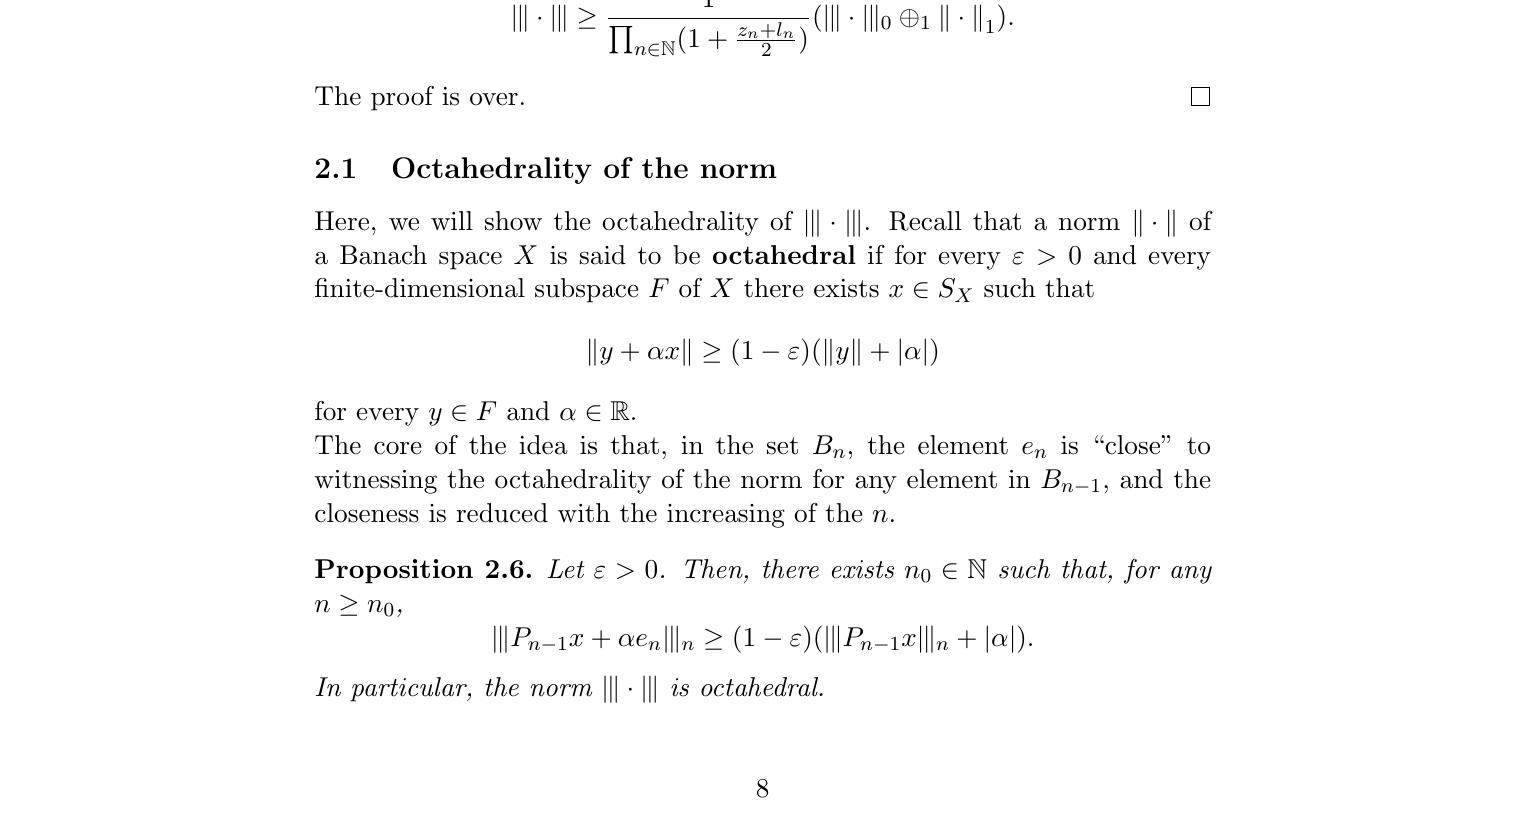
\includegraphics[width=\textwidth]{figures/supporting_tail_estimate_crop.png}
\end{center}

\section{A small smooth strictly convex norm}

\begin{lemma}\label{lem:h}
In the setting of Lemma~\ref{lem:CH}, there exists a continuous norm $h$ on
$X$ such that:
\begin{enumerate}
\item $h$ is strictly convex and G\^ateaux smooth;
\item $h(e_n)=2^{-n}$ for every $n$;
\item for $p\in P_{n-1}X$ and $\beta\in\R$,
\begin{equation}\label{eq:orth}
 h(p+\beta e_n)^2=h(p)^2+4^{-n}\beta^2,
 \qquad\text{hence }h(p+\beta e_n)\ge h(p).
\end{equation}
\end{enumerate}
The norm $h$ need not be equivalent to the original norm.
\end{lemma}

\begin{proof}
The restriction $N_0=N|_{X_0}$ is an equivalent G\^ateaux-smooth norm on the
separable space $X_0$.  Choose a weak-star dense sequence
$(\varphi_k)_{k\ge1}$ in $B_{X_0^*}$ and put
\[
 q_0(x_0)=\left(\sum_{k\ge1}4^{-k}|\varphi_k(x_0)|^2\right)^{1/2}.
\]
Weak-star density makes $(\varphi_k)$ separating, so $q_0$ is a norm.  It is
continuous and is the pullback of the Hilbert norm under the injective map
$x_0\mapsto(2^{-k}\varphi_k(x_0))_k$.  Consequently $q_0$ is strictly convex
and G\^ateaux smooth away from zero.  The norm
\[
                         r_0=N_0+q_0
\]
is equivalent and G\^ateaux smooth.  It is strictly convex: equality in its
triangle inequality forces equality for $q_0$, hence the two images in the
Hilbert space are positive collinear, and injectivity gives positive
collinearity in $X_0$.

For $x=x_0+\sum_{j\ge1}a_je_j$, define
\begin{equation}\label{eq:h}
 h(x)=\left(r_0(x_0)^2+\sum_{j\ge1}4^{-j}|a_j|^2\right)^{1/2}.
\end{equation}
The series term is bounded by a constant times $\|(a_j)\|_1^2$, so $h$ is
continuous on $X_0\oplus\ell_1$; injectivity makes it a norm.  It is the
$\ell_2$-sum of two strictly convex norms, hence strictly convex.

For smoothness, $r_0^2$ is G\^ateaux differentiable everywhere (with
derivative zero at the origin), and the weighted quadratic form in
\eqref{eq:h} is differentiable.  Away from the origin their sum is positive,
so composing with the square root proves G\^ateaux smoothness of $h$.
Finally, $h(e_n)=2^{-n}$ and \eqref{eq:orth} follows by separating the
$n$th coordinate in the defining sum.
\end{proof}

\section{Main partial theorem}

\begin{theorem}\label{thm:main}
Every separable real Banach space containing a complemented copy of $\ell_1$
admits an equivalent norm which is simultaneously
\begin{enumerate}
\item rotund,
\item G\^ateaux smooth, and
\item octahedral.
\end{enumerate}
In particular, the unit sphere of this norm has no LUR point.
\end{theorem}

\begin{proof}
The source paper already supplies a G\^ateaux-smooth equivalent norm on every
separable space \cite[Theorem~3.3]{DPS}; hence Lemma~\ref{lem:CH} applies.
Let $N$ be its Cobollo--H\'ajek norm, let $h$ be given by
Lemma~\ref{lem:h}, and set
\[
                              M(x)=N(x)+h(x).
\]
Because $N$ is equivalent and $h$ is continuous, $M$ is an equivalent norm.
It is G\^ateaux smooth as a sum of G\^ateaux-smooth norms.  If equality holds
in the triangle inequality for $M$, it must hold separately for both
summands.  Equality for the strictly convex norm $h$ forces positive
collinearity.  Thus $M$ is rotund.

It remains to prove octahedrality.  Fix a finite-dimensional subspace
$F\subset X$ and $0<\eps<1$.  Put $\eta=\eps/4$.  The projections $P_n$
converge strongly to the identity and therefore uniformly on the compact
$M$-unit sphere of $F$.  Taking $n$ sufficiently large, we have simultaneously
\begin{align}
 M((I-P_{n-1})y)&\le\eta M(y) &&(y\in F),\label{eq:tailF}\\
 N(P_{n-1}x+\beta e_n)&\ge(1-\eta)
       \bigl(N(P_{n-1}x)+|\beta|\bigr) &&(x\in X,\ \beta\in\R),\label{eq:Ntail}\\
 \frac1{1+2^{-n}}&\ge1-\eta.\label{eq:cn}
\end{align}
The middle line is \eqref{eq:CHtail}.  Since
\[
 M(e_n)=N(e_n)+h(e_n)=1+2^{-n}=:c_n,
 \qquad u_n:=e_n/c_n\in S_{(X,M)},
\]
we test octahedrality with $u_n$.

Take $y\in F$, $\alpha\in\R$, put $p=P_{n-1}y$, and let
$E=M(y-p)\le\eta M(y)$.  By the reverse triangle inequality,
\eqref{eq:Ntail}, and \eqref{eq:orth},
\begin{align*}
 M(y+\alpha u_n)
 &\ge M(p+\alpha u_n)-E\\
 &\ge (1-\eta)\left(N(p)+\frac{|\alpha|}{c_n}\right)+h(p)-E\\
 &\ge (1-\eta)\left(M(p)+\frac{|\alpha|}{c_n}\right)-E\\
 &\ge (1-\eta)\left(M(y)-E+(1-\eta)|\alpha|\right)-E\\
 &\ge (1-3\eta+\eta^2)M(y)+(1-\eta)^2|\alpha|.
\end{align*}
For $\eta=\eps/4$, both coefficients on the last line are at least
$1-\eps$.  Hence
\[
 M(y+\alpha u_n)\ge(1-\eps)\bigl(M(y)+|\alpha|\bigr)
 \qquad(y\in F,\ \alpha\in\R),
\]
which proves octahedrality.

Finally fix $x\in S_{(X,M)}$.  Applying octahedrality to
$F=\operatorname{span}\{x\}$ with errors tending to zero gives
$v_k\in S_{(X,M)}$ such that
\[
 M(x+v_k)\longrightarrow2,
 \qquad M(x-v_k)\longrightarrow2.
\]
The first convergence is the LUR test at $x$, while the second prevents
$M(x-v_k)\to0$.  Thus $x$ is not LUR.  Since $x$ was arbitrary, the sphere has
no LUR points.
\end{proof}

\section{Upgrade attempts and remaining obstruction}

The following focused strengthening attempts were checked before stopping at
Theorem~\ref{thm:main}.

\begin{enumerate}
\item \textbf{All separable spaces via octahedrality.}  This cannot work:
octahedral renormability is equivalent to containing $\ell_1$, as recalled in
\cite{CH}.  Reflexive examples such as $\ell_2$ therefore require a different
mechanism.

\item \textbf{Remove complementability but retain smooth octahedrality.}
Cobollo--H\'ajek explicitly identify removal of complementability as an open
extension of their theorem \cite[p.~2]{CH}.  Solving that extension would
enlarge the present theorem to separable spaces containing an arbitrary copy
of $\ell_1$, but would still not settle all separable spaces.

\item \textbf{Perturb an arbitrary octahedral norm.}  A compact injective
Hilbertian norm can be made small along a selected sequence, but an arbitrary
octahedral norm does not automatically provide one common witness sequence
with the uniform projection estimate needed above.  Moreover, smooth
octahedral renormability itself is unavailable without the preceding open
extension.  This route was not promoted.

\item \textbf{Use an equivalent strictly convex perturbation.}  Its value on
the $N$-unit vectors $e_n$ is bounded below, so normalization creates a fixed
loss and the octahedral constant need not tend to one.  The non-equivalent but
continuous norm $h$ in Lemma~\ref{lem:h} is the repair: $N+h$ remains
equivalent while $h(e_n)\to0$.
\end{enumerate}

These checks leave no credible path from the present mechanism to the exact
all-separable statement.  Theorem~\ref{thm:main} is therefore promoted as a
partial result rather than overstated as a full solution.

\section{Verification, novelty, and limitations}

\paragraph{Proof audit.}
The estimate was checked at the three interfaces where a perturbation argument
can fail: (i) $h$ is a genuine injective norm but is intentionally not
equivalent; (ii) $M=N+h$ is nevertheless equivalent; and (iii) the
normalization factor $c_n=1+2^{-n}$ and the finite-dimensional tail error are
both retained explicitly.  The final coefficients are
$1-3\eta+\eta^2$ and $(1-\eta)^2$, so $\eta=\eps/4$ is sufficient.  No
computational experiment is used as evidence.

\paragraph{Bounded novelty check.}
On 11 August 2026, the run's registry, solution, attempt, and proof-gap indexes
were searched for arXiv:2402.13869 and the phrases
``rotund octahedral'', ``strictly convex octahedral G\^ateaux smooth'', and
``complemented $\ell_1$ no LUR points''.  External arXiv/web searches used the
same close variants and also inspected arXiv:2408.03737 and arXiv:2410.18473.
No source stating the simultaneous rotund--G\^ateaux-smooth--octahedral
conclusion for complemented-$\ell_1$ spaces was located.  The decisive later
input \cite{CH} states smooth octahedrality, but not rotundity or the
nowhere-LUR conclusion.  This is a bounded search, not a claim of exhaustive
novelty; novelty confidence is moderate.

\paragraph{Limitations and review recommendation.}
The argument is written for real Banach spaces, matching the real-coordinate
tail inequality used in \cite{CH}.  It assumes a complemented copy of
$\ell_1$ and does not address separable spaces without such a copy.  Expert
review should focus on (a) the strict convexity and differentiability of the
auxiliary norm $h$, (b) the passage from the cited finite-stage notation to
\eqref{eq:CHtail} on $X$, and (c) the uniform finite-dimensional projection
estimate in \eqref{eq:tailF}.  If these checks pass, record this as a new
substantial positive class for Problem~3.7, not as a full solution.

\begin{thebibliography}{9}

\bibitem{DPS}
C.~A. De~Bernardi, A.~Preti, and J.~Somaglia,
\emph{A note on smooth rotund norms which are not midpoint locally uniformly
rotund}, arXiv:2402.13869 (2024).

\bibitem{CH}
Ch.~Cobollo and P.~H\'ajek,
\emph{Octahedrality and G\^ateaux smoothness},
arXiv:2408.03737 (2024); J. Math. Anal. Appl. 543 (2025).

\end{thebibliography}

\end{document}
